\chapter{2006 North American Monsoon Case Study --- Part II} \label{ch:2006_5}
\ifpdf
    \graphicspath{{Chapter_2006/figures/PNG/}{Chapter_2006/figures/PDF/}{Chapter_2006/}}
\else
    \graphicspath{{Chapter_2006/figures/EPS/}{Chapter_2006/}}
\fi

Previous studies have identified upper tropospheric enhancements of ozone associated with the monsoons above North America,
\citep[][and references therein]{Li:2005ss,Cooper:2009nx}, Asia \citep{Park:2007bh,Worden:2009ve},
and equatorial Africa \citep{Bouarar:2011ly} during summers.
\citet{Cooper:2007cr} calculated an ozone enhancement of 29--52~ppbv between 10--11~km
above Huntsville, Alabama. The observed upper tropospheric ozone enhancement has
been linked to the North American Monsoon (NAM) anticyclonic circulation, which traps ozone
precursors that subsequently enhance ozone production \citep{Li:2005ss}. \citet{Cooper:2009nx}
showed that more than 80\% of the upper tropospheric NO$_\mathrm{x}$
($\equiv\mathrm{NO}+\mathrm{NO_2}$) within the enhancement
is due to lightning, and that it is responsible for 25--30~ppbv ozone at 250~hPa. Furthermore,
it has been estimated that the ozone enhancement generates a positive radiative forcing of about
0.50~W\,m$^{-2}$ \citep{Cooper:2007cr,Choi:2009bh}. While these studies presented an overarching
picture to explain the formation of the enhanced ozone and quantify its consequences, the details
of the underlying physical and chemical processes remain unexplored. These previous studies also
did not examine the nonlinearity
of the sensitivity of ozone to the lightning-generated $\mathrm{NO_x}$ ($\mathrm{LNO_x}$) tested.

This chapter examines the upper tropospheric ozone enhancement's spatial and
temporal structures to quantify the advective, chemical, convective transport, and vertical
mixing tendencies of upper tropospheric ozone during the North American Monsoon.
Because of the importance of $\mathrm{NO_x}$ \citep{Cooper:2009nx}
and the uncertainty in the budget of $\mathrm{LNO_x}$ \citep{Schumann:2007fk}, this study focuses
on analyses pertaining to the potential effects of $\mathrm{LNO_x}$
on the ozone enhancement and addresses the following questions:
\begin{enumerate}
\item What is the vertical structure of the ozone chemical tendency? In order words,
at which levels are ozone being produced?
\item How does ozone chemistry respond to changes in $\mathrm{LNO_x}$ emission?
\item What are the secondary effects of the response of ozone chemistry on $\mathrm{LNO_x}$ emission?
\end{enumerate}

\section{Model and methods}\label{sect:model}

\subsection{Model setup}

% Ozone map
\begin{wrapfigure}{o}{0.5\textwidth}
	\centering
	\begin{singlespacing}
	\vspace{-.4in}
	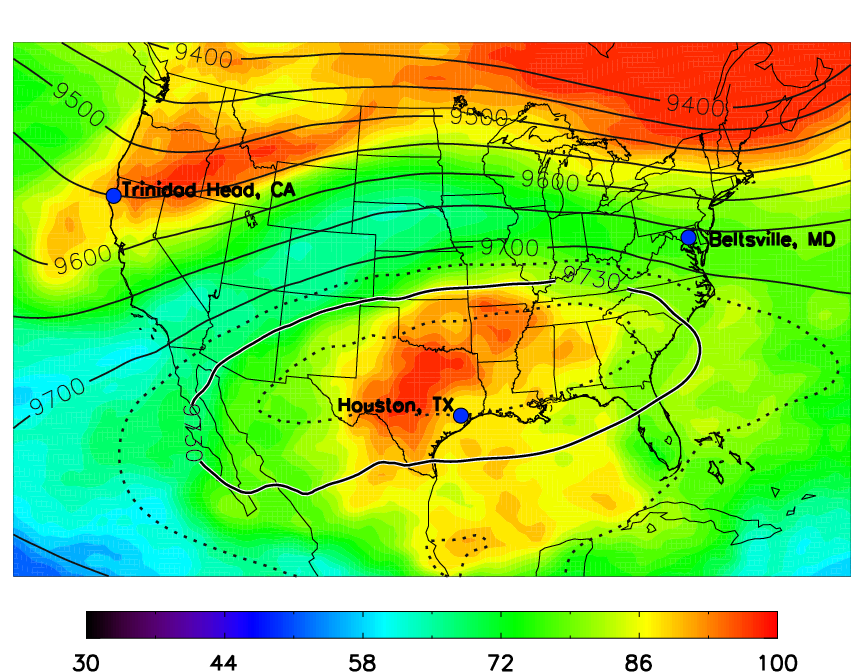
\includegraphics[width=0.48\textwidth]{Figures/o3_map.png}
	\caption[Simulated August mean ozone and geopotential heights at 300~hPa]{{\small
	Simulated ozone (ppbv) and geopotential height (m) at 300~hPa averaged for August 2006. The three locations indicated on the map
	are used for the tendency analysis in Section~\ref{sect:tendency}.}}
	\label{fig:o3_map2}
	\end{singlespacing}
\end{wrapfigure}

Figure~\ref{fig:o3_map2} shows the model domain for the WRF-Chem simulation performed
for the 2006 North American Monsoon case study at 36~km horizontal grid size. Meteorology
is initialized and nudged by the NCEP GFS reanalysis data.The Grell-3 convective
parameterization scheme, a modified version of the \citet{Grell:2002bs} scheme, is used.
In our simulations, the convective scheme is the primary source of precipitation.
From this, we use the level of neutral buoyancy, reduced by 2~km \citep{Wong:2013vn},
as the cloud top height input for the
\citet{Price:1992wb} lightning parameterization and scale the resulting flash rate down by a factor of 10 to obtain flash rates within $\sim7\%$ of
the National Lightning Detection Network \citep[NLDN;][]{Cummins:2009aa} observations.

The Regional Acid Deposition Model \citep[RADM2;][]{Stockwell:1990ez} is used for
the chemical mechanism with the fast Tropospheric Ultraviolet-Visible
\citep[FTUV;][]{Tie:2003ve} photolysis scheme. Boundary and initial chemical conditions are defined
by outputs from the Model for OZone and Related chemical Tracers (MOZART-4)
global chemistry model \citep{Emmons:2010fk}.
Additional model physics and chemistry options, as well as evaluation against
in-situ and remote sensing observations are described in the previous chapter.

\subsection{Diagnostic Outputs}

In addition to the standard meteorological and chemistry outputs, we produced additional
diagnostics computed within the model to aid our analysis.
Three passive tracers representing the lateral boundaries (BC), the boundary layer (BL), and the
stratosphere (ST) are used for air mass sourcing. These tracers are set to $1.0$ at their respective
sources (at the lateral domain boundaries, below the boundary layer height, and above
the tropopause) at every time step. In the previous chapter, these
tracers have been used to highlight that the anticyclonic monsoonal circulation prevents
ozone-poor air from the western domain boundary from entering the anticyclone region,
defined as the area with August mean geopotential height at 300~hPa greater than  9730~m.
A LNO$_\mathrm{x}$ tracer is also emitted with the LNO$_\mathrm{x}$ emission. Each of the four tracers has a
decaying twin with a lifetime of 24~hours. These tracers are
transported by advection, convective transport, and mixing. In this chapter, we use these
tracers to indicate, at specific locations, when $\mathrm{LNO_x}$, BL, and ST air
is influencing the modeled air mass composition.

To diagnose what physical and chemical processes are contributing to the ozone variability in
the upper tropospheric anticyclone, we have decomposed the tendency equation into its
component operators $\mathcal{P}$: horizontal advection ($\mathbf{v}\cdot\nabla$), vertical advection ($w\delta_z$),
convective transport ($\Delta_{\mathrm{conv}}$), vertical mixing/dry deposition ($\Delta_{\mathrm{vmix}}$),
net chemical productions/losses ($\Delta_{\mathrm{chem}}$), emission ($E$), and other loss
processes otherwise unspecified by the first five components such as wet deposition ($L$).
Therefore, we may write the change of the mixing ratio of a chemical constituent $C$ from time step $t$ to $t+1$
as follow:
\begin{equation}\label{eqn:fulltendency}
C^{(t+1)}-C^{(t)} = (\Delta_{chem}+\Delta_{conv}+\Delta_{vmix}+
\mathbf{v}\cdot\nabla+w\delta_z)C^{(t)}\delta t + E_C^{(t)}+LC^{(t)}
\end{equation}
We accumulate at every single time step the total tendency $T$ for a chemical species $C$ due to a single process $p$ up
to time $t$ from initialization:
\begin{equation}\label{eqn:tendency}
T_p^{(t)}=\sum_{\tau=0}^{t-1}\Delta_pS^{(\tau)}\delta\tau
\end{equation}
All processes include nonlinear terms associated with the respective solver. The decoupled advective
components are extracted from within the WRF dynamic core, while convective, vertical mixing, and chemical
tendencies are computed by differencing the mixing ratios before and after their respective solver. Thus,
no information is lost during the accumulation process. If
$\langle E_C^{(\tau)}+LC^{(\tau)}\rangle_{\tau<t}=0$,
we may expect $\sum_{p\in\mathcal{P}}T_p^{(t)}\equiv C^{(t)}-C^{(0)}$ to hold.
In the upper troposphere, emission (except for lightning-generated NO) should be zero as aircraft
emission is not included in the simulations, and wet deposition of the species of interest (O$_3$, CO,
$\mathrm{NO_x}$) is negligible. Thus the first five processes in Equation~\ref{eqn:tendency}
should be sufficient in capturing the full tendency of these chemical constituents.

\section{Tendency evalution}\label{sect:tendency}

For the following analyses, we will be focusing on the three locations shown in Figure~\ref{fig:o3_map2}.
The first location,  Trinidad Head, California (40.80$^\circ$N, 124.15$^\circ$W), represents the
continental inflow region, which is largely unaffected by conditions and air masses from within the
anticyclone or contiguous United States (CONUS) in general. The modeled August average O$_3$ and geopotential heights
show that Trinidad Head can have high O$_3$ due to stratospheric air just to the north
(Figure~\ref{fig:o3_map2}) and remains outside of the anticyclone region.
The second location is Houston, Texas (29.72$^\circ$N,
95.40$^\circ$W), representing the anticyclone region, which is the primary subject for this study.
The third location, Beltsville, Maryland (39.04$^\circ$N, 76.52$^\circ$W), represents
the continental outflow region, which periodically receives air from the jet and
the anticyclone (Figure~\ref{fig:o3_map2}).

\newpage\subsection{Temporal variability}

% Tendency residuals
\begin{wrapfigure}{o}{0.5\textwidth}
	\centering
	\begin{singlespacing}
	\vspace{-.3in}
	\includegraphics[width=0.48\textwidth]{Figures/tendency_res.eps}
	\caption[Ozone total, advective, and residual tendencies]{{\small
	Ozone total tendencies (black lines) between 200--600~hPa, (a) horizontal (red) and vertical (blue) advective tendencies and (b)
	residual tendencies (red line) after removing advective components.}}
	\label{fig:tend_res}
	\end{singlespacing}
\end{wrapfigure}

The primary sources for local temporal variability are horizontal advection and vertical advection.
Figure~\ref{fig:tend_res} shows the advective tendencies for ozone during August near Houston
between 200--600~hPa, which includes mid-to-upper troposphere and encompassing altitudes covered by
the remaining analyses performed in this study. Both the horizontal and vertical components are often the same
magnitude as the total tendency. However, the combined advective tendency is frequently much
smaller because the two components often have opposite signs. The residual
tendency, i.e. the total ozone tendency without the two advective components, is the combined
chemical, convective, and vertical mixing tendencies.
It is useful to note that, because the components are not restricted to be either positive or negative,
removing a tendency due to a specific process from the total tendency does not guarantee a smaller
residual. In addition, while the time series shown is from Houston, the same results are applicable
to the advective tendencies at other locations.

% Tendency timeseries
 \begin{figure}
 \noindent\includegraphics[width=40pc]{Figures/tendency_ts.eps}
 \caption[Ozone mixing ratios, tendencies, and passive tracer time series]{\small
\textbf{Ozone mixing ratios, tendencies, and passive tracer time series} ---
Time series at (a) Trinidad Head, (b) Houston, and (c) Beltsville
showing the minimum-mean-maximum ozone time series (black) between
270--330~hPa overlaid with IONS-06 ozonesonde measurements
represented as red vertical lines for the range and solid $\diamondsuit$
for the mean value. Ozone chemical (red) and convective (blue) tendency
components are given according to the right axis labels in units
of ppbv accumulated for every 3-hourly output interval. Boundary layer (BL, blue)
and stratospheric (ST, red) decaying tracers are
given in \%. LNO$_{\mathrm{x}}$ decaying tracer (green) is given in ppbv.}
 \label{fig:tend_ts}
 \end{figure}

To characterize the residual tendency at the 300~hPa level, we examine the remaining
components of the tendency accumulation equation (Eqn.~\ref{eqn:fulltendency}) at the three
locations between 270--330~hPa. All results are computed using the nearest $11\times11$ model grids to the IONS-06 site location.
We find that the vertical mixing tendency is usually more than an order of magnitude smaller than the
chemical and convective tendencies at this altitude, thus vertical component is omitted from the
analysis and Figure~\ref{fig:tend_ts}. In addition to the time series of the two tendency components,
Figure~\ref{fig:tend_ts} shows the ozone mean mixing ratios and the range between its minimum and maximum values. To put into
perspective the skill of the model in simulating the variability, distributions of ozonesonde measurements
between 270 and 330~hPa from the IONS-06 campaign \citep{Thompson:2008rp} are
overlaid on top of the model results. At the bottom of each panel, boundary layer (BL), stratospheric
(ST), and lightning (LNO$_{\mathrm{x}}$) decaying tracers are included to indicate time periods
when these sources influenced the upper troposphere above each location.

Trinidad Head occasionally receives stratospheric ozone from the northern latitudes as evident in the ST tracer, which is
responsible for the high ozone simulated for particular days
(e.g. August 2 and August 7). The largest 3-hourly chemical tendency for Trinidad Head is
$0.35$~ppbv per 3~hours. This can be compared to that for advection, which has a mean
3-hourly absolute advective tendency of 82.8~ppbv. The accumulated August chemical
tendency, including both positive and negative phases, is 0.096~ppbv, this can be compared
to $-2.0$~ppbv for convective transport, 8.1~ppbv for vertical mixing, and $-135$~ppbv for
the two advective tendencies combined. The large value from the advective tendency
is the result of a high stratospheric ozone phase over Trinidad Head at the beginning of August
and a low stratospheric ozone phase at the end of August. Thus, the ozone at Trinidad Head is
controlled by the advective tendencies with vertical mixing and convective transport providing
small contributions. The chemical tendency is negligible at this location.

Above Houston, August began with an event of high stratospheric contribution ($\sim0.1\%$ decaying ST) to O$_3$
and ended with negligible stratospheric contributions ($<10^{-4}\%$), thus resulting in a large accumulated total
of $-133$~ppbv despite a large range of values if integrated for other periods.
Chemistry is much more important here than Trinidad Head, the minimum/maximum chemical tendencies
are $-6.4$/6.8~ppbv per 3~hours, a 20-fold increase from that in the continental inflow region.
Moreover, the August total change due to chemical production is 80~ppbv, which is 3 orders
of magnitude higher that that at Trinidad Head. The total convective tendency is also higher, with an
August accumulated value of positive 12~ppbv.
As will be shown in the next section, 300~hPa is well below the simulated main convective outflow level
and experiences increases in ozone due to subsidence. Vertical mixing is substantially smaller (2~ppbv)
due to generally smaller vertical gradients at 300~hPa above the southern United States. During
August 23--26,  there are large convective transport and chemical tendencies. This event coincides with
enhanced LNO$_{\mathrm{x}}$ and BL tracer values. However, due to comparably strong
O$_3$ chemical losses, the accumulated total is much less than it would be otherwise.

Upper tropospheric air above Beltsville experienced $-2.4$/3.8~ppbv of minimum/maximum 3-hourly O$_3$ chemical
tendency, with an August accumulated net change of 59~ppbv of O$_3$ due solely to chemistry.
This value can be compared to the accumulated change due to convection
(7.5~ppbv), vertical mixing (4.3~ppbv), and advection ($-73$~ppbv). Unlike Houston, however,
Beltsville also shares some characteristics with Trinidad Head, both of which periodically
receive high stratospheric ozone (e.g. August 8--13).

\subsection{Vertical structure}
% Tendency vertical profiles
 \begin{figure}
 \noindent\includegraphics[width=40pc]{Figures/tendency_v.eps}
 \caption[August average mixing ratio and tracer vertical profiles]{\small
August average vertical profiles at (a) Trinidad Head, (b) Houston, and (c)
Beltsville. Dashed lines are the mean 1-day decaying tracers for BL (blue, \%),
ST (red, \%), and LNO$_{\mathrm{x}}$ (green, ppbv) according to the
values on the top axis. Solid lines are the accumulated chemical
tendency (red), convective tendency (blue), and the mean ozone profile
(black) in ppbv according to the values of the bottom axis. The closest
$11\times11$ grid points to each IONS-06 site are averaged to compute
these profiles.}
 \label{fig:tend_v}
 \end{figure}

While the time series analysis above, focusing at the pressure level (270--330~hPa) investigated by \citet{Li:2005ss}
(300~hPa) and near that by \citet{Cooper:2007cr} (250~hPa), shows interesting variabilities,
the vertical structure is not represented. Due to convective entrainment/detrainment, selected
pressure levels can experience drastically different chemical properties. In the following
analysis, we examine the August mean vertical structures of the chemical and convective
tendency components (Figure~\ref{fig:tend_v}). As in the previous section, the ozone
mixing ratios and passive tracer values are also provided to give context.

The continental inflow region (Trinidad Head) lacks both BL and LNO$_{\mathrm{x}}$
tracers in the upper troposphere. Despite having higher ozone mixing ratios than the
other two locations, the accumulated chemical tendency remains low with a maximum of
$19.4\pm2.4$~ppbv at 205~hPa, which is above the level of maximum
convective outflow (300~hPa) at Trinidad Head. Because of the lack of
LNO$_{\mathrm{x}}$ emission and  in-situ chemical production,
the ozone mixing ratio remains low between stratospheric intrusion or episodes of lowered tropopause, allowing
the air to remain relatively ``clean'' until reaching Minnesota (Figure~\ref{fig:o3_map2}). This influx of low-ozone, 
chemically-``slow'' air mass is responsible in generating the oval-shaped ozone
enhancement that outlines the northwestern edge of the mean NAM circulation.

At Houston, near the center of the mean-state anticyclonic circulation, both the ozone
chemical and convective tendencies are substantially higher than Trinidad Head. At
200~hPa, Houston experiences an August total change of $109\pm17$~ppbv due
solely to chemistry, about 5 times higher than that in Trinidad Head.
The largest O$_3$ chemical production occurs during the day, and is often partially balanced by O$_3$
chemical loss at night.
On the other hand, ozone-poor air and BL tracers are transported into
the upper troposphere through convection, detraining primarily at 145~hPa with a
net change of $-172$~ppbv O$_3$ during August, in part caused by a nearby outlier
with $-1092$~ppbv during the same period. The localized high convective tendency is
an indication for stationary features such as convection triggered by coastlines
or orography.

Beltsville, situated in the continental outflow region, shows small convective
tendencies, with a peak at 175~hPa, but BL tracers and chemical tendencies are comparable to those at Houston.
At the same time, Beltsville also experiences periodically high stratospheric ozone events
in the upper troposphere similar to those at Trinidad Head. With these diagnostics,
it can be inferred that the primary source for ozone precursors, including
LNO$_{\mathrm{x}}$ in the continental outflow region is the advective influx from
upwind regions rather than vertically transported from the local boundary layer
via convection. This is contrary to that within the anticyclone, where chemical
production of ozone in the upper troposphere is enhanced by precursor sources
located directly below at the boundary layer, as indicated by the simultaneous
enhancements in both convective transport and chemical tendencies. An in-depth analysis of the ozone
budget and variability at Beltsville and New England can be found in
\citet{Thompson:2007gd,Thompson:2007ov}, wherein data from IONS-4, the
predecessor of IONS-06, are utilized. They found that tropospheric ozone in
northeastern North America was composed of 10--15\% BL sources, 10--15\%
regional sources including lightning, 20--25\% stratospheric ozone, and
$\sim50\%$ recently advected or aged air from elsewhere. While we
do not produce exact values, the rankings from their study and those found in
the present study for Beltsville are largely consistent.

\section{Sensitivity to lightning}\label{sect:sensitivity}

\subsection{Spatial distribution}

% Lightning sensitivity -- maps
 \begin{figure}
 \noindent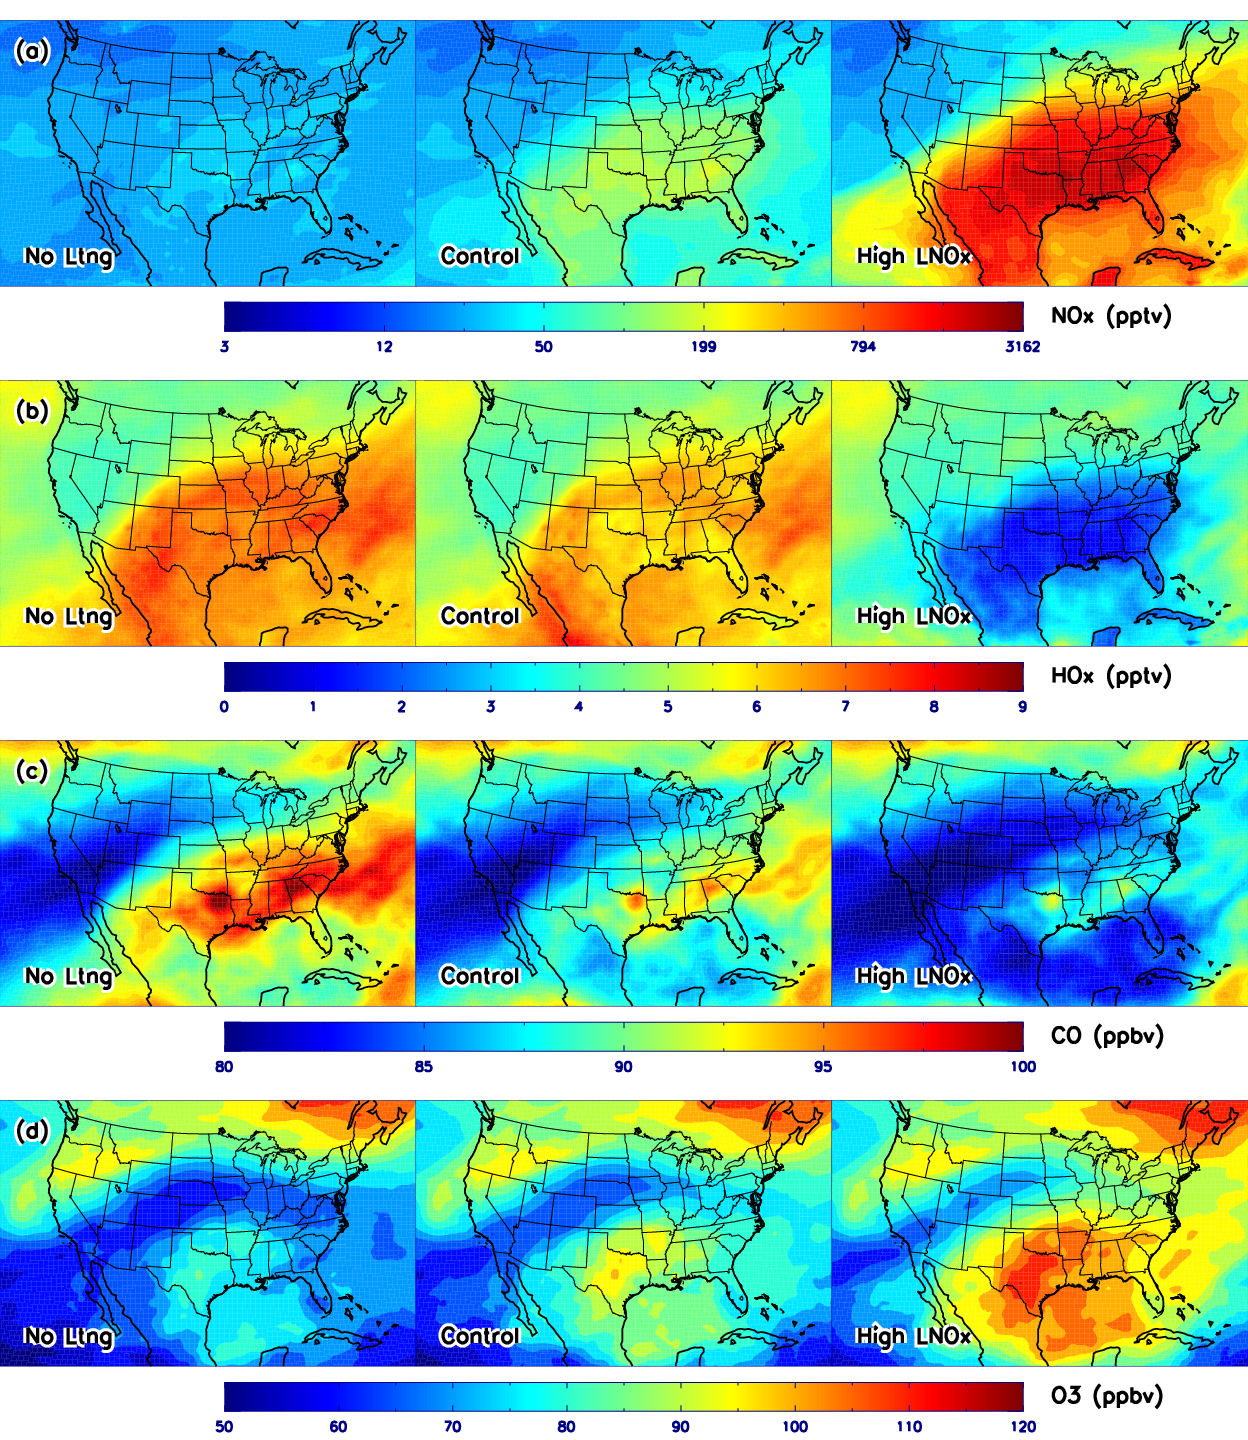
\includegraphics[width=40pc]{Figures/ltngsens_map.png}
 \caption[Sensitivity of various species to \chem{LNO_x} at 300~hPa]
{\small Model simulated mean (a) NO$_{\mathrm{x}}$, (b) HO$_{\mathrm{x}}$,
(c) CO, and (d) O$_3$ for no-lightning (left column), control (center
column), and high-LNO$_{\mathrm{x}}$ (right column) scenarios at 300~hPa
during August. Note that NO$_{\mathrm{x}}$ is contoured on a log scale
while the rest are contoured on linear scales.}
 \label{fig:ltng_map}
 \end{figure}

\citet{Cooper:2007cr} attributed much of the enhanced upper tropospheric ozone in the
anticyclone to $\mathrm{NO_x}$ produced by lightning. To understand the how LNO$_{\mathrm{x}}$
affects the ozone enhancement, we compare results from the control simulation, i.e.
the simulation used in the previous section, to two additional sensitivity simulations.
The first sensitivity simulation is a no-lightning case, where the lightning $\mathrm{NO_x}$ emission is suppressed entirely.
The second sensitivity simulation is a high-$\mathrm{LNO_x}$ case, where lightning flash rate is 10 times greater
than the control case. This scenario tests the case wherein model may substantially underestimate $\mathrm{LNO_x}$
with the potential of $\mathrm{NO_x}$-titration, which has been measured within convective outflows of large
storms \citep[e.g.][]{Stith:1999fk,Ridley:2004oa,Ott:2007hs,Cummings:2013vn}. The resulting mean spatial
distributions of NO$_{\mathrm{x}}$, HO$_{\mathrm{x}}$, CO, and O$_3$ at 300~hPa
during August are shown in Figure~\ref{fig:ltng_map}.

Although the no-lightning scenario shows higher ozone within the anticyclone compared to the immediate surrounding
areas, there is an overall low bias compared to ozone observations (see previous chapter).
In comparing results from the different simulations, we find
NO$_{\mathrm{x}}$ is substantially increased within the anticyclone above background values in the Pacific Northwest
region from $31.6\pm4.5$~pptv to $135\pm35$~pptv in the control case
and 1680$\pm540$~pptv in the high-$\mathrm{LNO_x}$ case.
The contribution of total NO$_{\mathrm{x}}$ mixing ratio from LNO$_{\mathrm{x}}$ can be calculated as,
$$
\Delta[\mathrm{NO_x}] = [\mathrm{NO_x}]-[\mathrm{NO_x}]_0 = (1-f)[\mathrm{LNO_x}]
$$
where $f$ is the fraction loss of $\mathrm{LNO_x}$ in the atmosphere due to
chemistry or deposition and $[\mathrm{NO_x}]_0$ is the $\mathrm{NO_x}$
mixing ratio without lightning. For small changes in the atmospheric composition, $f$ should be
constant and thus the addition of $\mathrm{LNO_x}$ is expected to linearly
increase $[\mathrm{NO_x}]$.
If one assumes that the change between no-lightning and control cases is linear, extrapolating
to the high-$\mathrm{LNO_x}$ case would give 1070~pptv, which is less than
the 1100--2200~pptv simulated. This is due to the decrease in $\mathrm{HO_x}$
(as discussed below), the primary reagent converting $\mathrm{NO_x}$ into
reservoir species, in response to increasing $\mathrm{LNO_x}$. Subsequently,
we have $\partial f/\partial[\mathrm{LNO_x}]<0$, resulting in a superlinear increase of $\mathrm{NO_x}$.

HO$_\mathrm{x}$ is substantially decreased with
increasing LNO$_\mathrm{x}$ emission. The initial August mean mixing ratio
at 300~hPa without lightning is $6.94\pm0.38$~pptv within the anticyclone. This
is larger than the $\sim$4--5~pptv in the Pacific Northwest and inflow regions. It
is slightly decreased to $6.27\pm0.37$~pptv in the control simulation, or a
10\% decrease from the no-lightning scenario. For the high $\mathrm{LNO_x}$
scenario, HO$_\mathrm{x}$ is further decreased to $1.80\pm0.59$~pptv, far
below the value of the Pacific Northwest, and is 71\% less than the
control simulation, which is a larger decrease than that would have been
obtained if one were to extrapolate the initial 10\% decrease with an
exponential model ($\sim61\%$). The decreasing  HO$_\mathrm{x}$ with
increasing NO$_\mathrm{x}$ is the result of its interactions with O$_3$,
NO$_\mathrm{x}$, and CO after production from $\mathrm{O(^1D)+H_2O}$,
which is presumably proportionally increasing with the increased level of
O$_3$.

Even though $\mathrm{CO+OH\rightarrow CO_2+HO_2}$ is the only
chemical loss pathway for CO specified in RADM2 and that HO$_\mathrm{x}$
is substantially decreased by a factor of 3.8 from no-lightning to high-$\mathrm{LNO_x}$,
CO is simulated to decrease with increasing lightning. Without
lightning, the August mean mixing ratio for CO is $92.8\pm2.8$~ppbv
within the anticyclone. This is reduced to $89.8\pm2.4$~ppbv for the control simulation
and $85.5\pm2.4$~ppbv for the high-$\mathrm{LNO_x}$ simulation.
The anti-correlation of CO with $\mathrm{LNO_x}$ is due to the primary
effect of reduced in-situ production of CO from various VOC oxidations
by OH.

Finally, O$_3$ is increased with increasing LNO$_\mathrm{x}$, consistent
with prior studies on this subject \citep[e.g.][]{Cooper:2007cr,Allen:2010fk}.  Ozone mixing ratio is increased from
$74.5\pm5.3$~ppbv to $86.4\pm6.7$~ppbv ($+16\%$) at 300~hPa, which is
a smaller increase than that found by \citet{Cooper:2007cr}. In the high-LNO$_{\mathrm{x}}$ case, averaged O$_3$ is
further increased to $101.1\pm6.8$~ppbv, a 26.6~ppbv or 36\% increase
relative to the no-lightning scenario. The reduced sensitivity of O$_3$ to LNO$_{\mathrm{x}}$
at higher flash rates indicates a negative feedback process at play
despite the superlinear increase in $\mathrm{NO_x}$ for the high-$\mathrm{LNO_x}$ scenario.

\subsection{Vertical structure}

Vertical distributions of species mixing ratios and tendencies are also affected by
the $\mathrm{LNO_x}$ emission factor. Figure~\ref{fig:ltng_vert} shows the vertical
profiles for O$_3$, CO, and NO$_\mathrm{x}$ and their tendencies from the three simulations
averaged within the anticyclone column. With the exception of O$_3$ and
NO$_\mathrm{x}$ in the high-LNO$_{\mathrm{x}}$ scenario, the shapes of the mixing
ratio vertical profiles are consistent across simulations. When considering only
the magnitude of changes, the greatest effect of LNO$_\mathrm{x}$ emissions
on ozone occurs in the 300--500~hPa layer. The ozone mixing ratio increases
by 33~ppbv in the control simulation compared to the no-lightning simulation.
The ozone chemical tendency for August also increases
substantially in this layer from $-29$~ppbv to $+187$~ppbv for the no-lightning to high-$\mathrm{LNO_x}$ cases.
On the other hand, despite having a LNO$_\mathrm{x}$
emission peak in the mid-troposphere as prescribed according to \citet{Ott:2010lo},
NO$_\mathrm{x}$ is enhanced most prominently at the $\sim170$~hPa level from
84~pptv to $\sim3$~ppbv. This increase, together with the reversal in ozone chemical
tendency at this level, suggests that NO$_\mathrm{x}$-titration potentially occurs.

% Lightning sensitivity -- vertical profiles
 \begin{figure}
 \noindent\includegraphics[width=40pc]{Figures/ltngsens_vert.eps}
 \caption[August mean mixing ratios and chemical tendencies]{\small
August mean mixing ratios and accumulated chemical tendencies
for (a) O$_3$, (b) CO, and (c) NO$_{\mathrm{x}}$ within the anticyclone
region for the no-lightning (green), control (blue),
and high-LNO$_{\mathrm{x}}$ (red) scenarios. Means are computed on model levels, and then
gridded by the mean pressure.}
 \label{fig:ltng_vert}
 \end{figure}

In all simulations, the August mean ozone chemical tendencies within the anticyclone
are positive in the boundary layer (BL) due to surface emissions, become negative just above
the BL, then become positive again in the mid-troposphere, and remain
positive up to the tropopause or higher. The mid-tropospheric altitudes at which the signs of the
accumulated chemical tendencies return to positive are due to positive production above a negative
background loss rate enhanced by LNO$_\mathrm{x}$. Without lightning, the
lowest level with a positive O$_3$ chemistry tendency in the free troposphere is $\sim340$~hPa.
In the control scenario, the switch from negative to positive chemistry tendency
drops to the $\sim470$~hPa level. This is further lowered to $\sim630$~hPa with the
high-LNO$_\mathrm{x}$ scenario. Thus, the vertical distribution of LNO$_\mathrm{x}$,
which impacts the vertical profile of ozone's sensitivity to the emission parameter,
can directly perturb the structure and vertical extent of the ozone enhancement
by influencing the level at which net ozone production is attained.

The mixing ratio of NO$_\mathrm{x}$ increases superlinearly in the upper troposphere due to
LNO$_\mathrm{x}$ emissions between the control and high-$\mathrm{LNO_x}$
simulations, as was discussed previously. Consequently, the presence of the exceedingly
high NO$_\mathrm{x}$ induces a decrease in the chemical production of
O$_3$. While NO$_x$-titration has been suggested to be possible during intense
thunderstorms \citep[e.g][]{Cummings:2013vn}, the persistent occurrence
of NO$_\mathrm{x}$-titration has not been observed and the result of this simulation is likely only an
artifact as a result of the 10-fold increase in lightning production, and is
further amplified by the reduced NO$_{\mathrm{x}}$ loss rate to HNO$_3$.

\subsection{Diurnal variabilities}

% Lightning sensitivity -- diurnal
\begin{wrapfigure}{o}{0.5\textwidth}
	\centering
	\begin{singlespacing}
	\includegraphics[width=0.48\textwidth]{Figures/ltngsens_diurnal.eps}
	\caption[Diurnal variability in tendency and mixing ratio frequency distributions]{{\small
	\textbf{Diurnal variability in tendency and mixing ratio frequency distributions} ---
	Distributions (5pct-mean-95pct) of chemical tendencies
	and mixing ratios for O$_3$, O$_{\mathrm{x}}$, CO, and the mixing ratio
	for HNO$_3$ between 150--300~hPa during August within the
	anticyclone. Nighttime (3--9~UTC) tendencies are represented by dashed
	lines while daytime (15--21~UTC) tendencies are represented by solid lines.}}
	\label{fig:ltng_di}
	\end{singlespacing}
\end{wrapfigure}

As shown in Figure~\ref{fig:tend_ts}, Houston experienced strong negative phases in its ozone chemical tendency,
which partially negated the accumulated daytime production. To determine the
response of ozone chemistry to lightning, it is thus necessary to take into account
daytime versus nighttime chemistry as not to include nocturnal loss into the budget
for daytime NO$_{\mathrm{x}}$-titration. To do so, Figure~\ref{fig:ltng_di} shows the
daytime ozone production separated from nighttime losses between 150--300~hPa within
the anticyclone. The daytime tendencies are extracted from 15--21~UTC and the
nighttime tendencies are extracted from 3--9~UTC. The diurnal variability in the
mean values of species mixing ratio are negligible, and thus only daytime values
are shown. Due to interconversion between O$_3$ and NO$_2$, we also examine
odd oxygen $\mathrm{O_x\equiv O_3+NO_2}$ instead of NO$_2$ in the following
analysis.

Without lightning, the mean daytime O$_3$ chemical tendency is $0.088$~ppbv/hr and the
95th-percentile is $0.259$~ppbv/hr. For the control case, the daytime mean
and 95-pct respectively increase to $0.353$~ppbv/hr and $0.904$~ppbv/hr.
However, further increasing LNO$_\mathrm{x}$ to the high-LNO$_\mathrm{x}$
scenario only slightly increases the mean ozone chemical tendency to $0.403$~ppbv.
Considering the combined all-day accumulated tendency, which decreased
between the two scenarios with lightning (Figure~\ref{fig:ltng_vert}a), it is apparent
that the nighttime loss phase plays in important role in modulating the total
response of ozone chemical tendencies to changes in the lightning emission factor.
Nonetheless, the lowered sensitivity in the daytime chemistry alone still supports
the conjecture that NO$_\mathrm{x}$-titration is occurring albeit not as strongly
as implied by Figure~\ref{fig:ltng_vert}a.

Comparing the changes in the distributions of chemical tendencies for
O$_3$ and O$_{\mathrm{x}}$, it is apparent that the bulk of the ozone losses in the
high-LNO$_{\mathrm{x}}$ scenario is due to conversion to NO$_2$. This is also
supported by the increase in HNO$_3$ from 6.6~ppbv in the control
case to 39.6~ppbv in the high-LNO$_{\mathrm{x}}$ case.

Without photolysis, the nighttime maximum O$_3$ tendencies are all
near zero. Thus, without net O$_3$ production, we can define zero as the baseline and evaluate
the sensitivities as relative changes. Without lightning, the ozone loss is 0.90~pptv/hr
with the 5th-percentile at 2.93~pptv/hr. The mean loss is increased to 5~pptv/hr
($5.6\times$) and the 5th-pct is increased to 25.8~pptv/hr ($8.8\times$) in
the control scenario. Increasing LNO$_\mathrm{x}$ by a factor of 10, the mean nighttime O$_3$ loss
is now 48.2~pptv/hr, a $9.5\times$ increase from the control simulation;
slightly-sublinear change relative to the increase in emission. Finally, the loss near the
left tail of the distribution increases linearly at both the 5th-percentile
($25.8\rightarrow259$~pptv/hr) and minimum ($0.179\rightarrow1.78$~ppbv/hr).

\subsection{NO$_\mathrm{x}$-titration}

While it is evident that the high-LNO$_\mathrm{x}$ scenario produces unrealistic
concentrations of NO$_\mathrm{x}$ in the troposphere, $>3$~ppbv of
NO$_\mathrm{x}$ has been observed within convective outflows of large
storms \citep[e.g.][]{Stith:1999fk,Ridley:2004oa,Ott:2007hs,Cummings:2013vn}. Thus it is useful to understand the
chemistry thresholds that triggered the negative response in ozone chemistry.
A steady-state analysis on ozone production and loss terms can be done
following the method outlined by \citet{Kleinman:1997vn}. In a photostationary steady-state, the radical
production rate $Q$ is equal to the total loss rate, characterized by radical-radical
reactions $L_R$ (e.g. $\mathrm{HO_2+HO_2}$) and radical-nitrogen reactions
$L_N$ (e.g. $\mathrm{NO_2+OH}$). That is, $Q=L_R+L_N$. The response of
ozone production to the available NO can then be quantified as follow
\citep{Kleinman:1997vn}:
\begin{equation}\label{eqn:kleinman}
\frac{d\ln P(\mathrm{O_3})}{d\ln[\mathrm{NO}]} =
\frac{1-3/2\,L_N/Q}{1-1/2\,L_N/Q}
\end{equation}
where $L_N/Q$ is the fraction of free radicals removed by NO$_\mathrm{x}$.
In the upper troposphere, $L_N$ and $L_R$ can be approximated by the
reaction rate of $\mathrm{NO_2+OH}$ and twice the rate of
$\mathrm{HO_2+HO_2}$, respectively. For consistency with the simulated chemistry,
all offline computations are conducted using the rate equations and parameters from RADM2
\citep[][and references therein]{Stockwell:1990ez}. Using August data points
at 15, 18, and 21~UTC within the anticyclone column between 150--250~hPa
and 350--450~hPa, the daytime reaction rates $L_N=k\mathrm{[NO_2][OH]}$ and
$L_R=2k'\mathrm{[HO_2][HO_2]}$ are plotted in Figure~\ref{fig:ltng_rxn}.
\citet{Kleinman:2001fk} showed that
a VOC-sensitive regime is in place when $L_N/Q>0.5$, compared to the NO$_\mathrm{x}$-sensitive regime
below this threshold. Further, $L_N/Q>2/3$ is favorable for NO$_\mathrm{x}$-titration,
i.e. production of ozone is expected to decrease with further increases in
NO$_\mathrm{x}$, as demonstrated by Equation~\ref{eqn:kleinman}. Thus,
if the majority of air masses lies above the $2/3$ threshold, an overall decrease
in ozone production or even net loss can be expected to occur.

% Lightning sensitivity -- Leighton
 \begin{figure}
 \noindent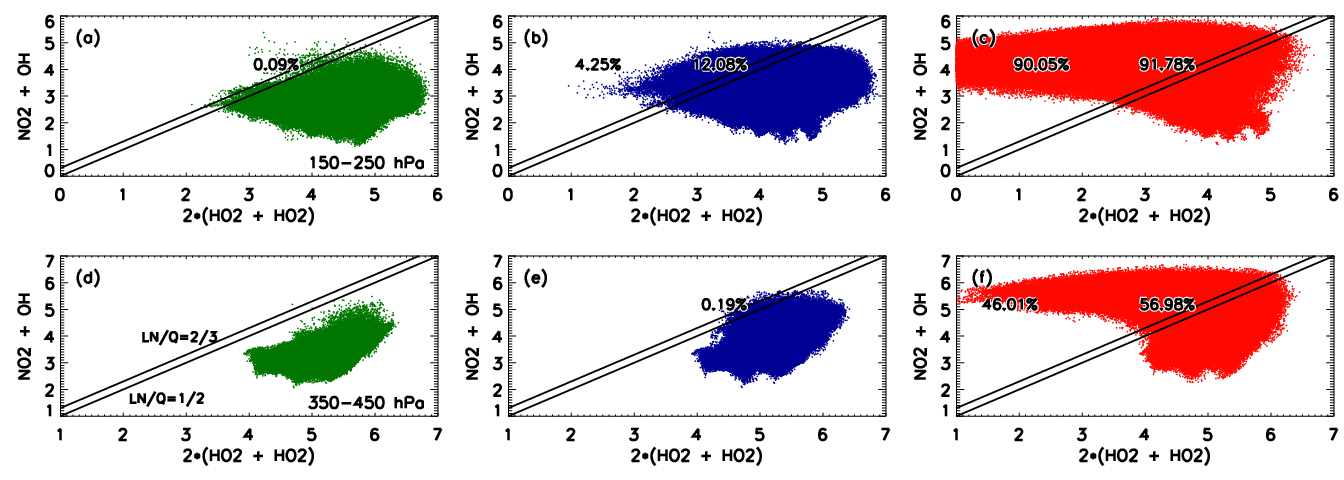
\includegraphics[width=40pc]{Figures/rxn.png}
 \caption[Daytime reaction rates]{Daytime reaction rates ($\log_{10}$~molec.~cm$^{-3}$~s$^{-1}$
for NO$_2+$OH and ($2\times$) HO$_2+$HO$_2$ at 150--250~hPa (a--c)
and 350--450~hPa (d--f) without lightning (a,d), control simulation (b,e),
and high LNO$_{\mathrm{x}}$ scenario (c,f). The left percentage (if present) is the fraction
of data points where $L_N/Q>2/3$. The right, or the only one, percentage (if present) is that
of $L_N/Q>1/2$.}
 \label{fig:ltng_rxn}
 \end{figure}

The percentage of data points where $L_N>L_R$, or $L_N/Q>1/2$, and
$L_N/Q>2/3$ are computed at both levels for all three sensitivity simulations. When
lightning is suppressed, nearly all data points lie within $L_N/Q<1/2$,
which means that the upper troposphere in the anticyclone is NO$_\mathrm{x}$-sensitive.
In the control simulation, about 12\% in the upper troposphere is VOC-sensitive,
but below 350~hPa almost all HO$_\mathrm{x}$ continues to
be terminated by radical-radical reactions. In the high-LNO$_\mathrm{x}$
simulation, 92\% and 57\% of the data points are within the VOC-limited regime
($L_N/Q>1/2$) for the two pressure ranges. The fraction of data points
where the expected response of $P(\mathrm{O_3})$ to [NO$_\mathrm{x}$]
is negative ($L_N/Q>2/3$) are 90\% for 150--250~hPa and 46\% for
350--460~hPa.

Thus, for a reasonable $\mathrm{LNO_x}$ emission scenario, i.e. similar to that
in our control case, 10\% or more of the upper tropospheric air mass is
VOC-sensitive and about 4\% is in the $\mathrm{NO_x}$-titration regime.

\subsection{Convective transport}

% Lightning sensitivity -- convective structure
\begin{wrapfigure}{o}{0.5\textwidth}
	\centering
	\begin{singlespacing}
	\vspace{-.4in}
	\includegraphics[width=0.48\textwidth]{Figures/ltngsens_o3conv.eps}
	\caption[Sensitivity of ozone convective tendency to \chem{LNO_x}]{{\small
	Vertical profiles of accumulated ozone convective tendency during August for the three
	lightning sensitivity simulations within the anticyclone column.}}
	\label{fig:ltng_conv}
	\end{singlespacing}
\end{wrapfigure}

The result of convective transport detrainment and mixing, i.e. convective tendency, depends
on the differences in ozone mixing ratios between model vertical levels. If entrainment occurs
at high ozone levels, detrainment at low ozone levels would be positive. On the contrary,
if low ozone levels are entrained and detrainment occurs at high ozone levels, convective
tendencies at the detrainment level would be negative.

Due to changes in the vertical profiles of mixing ratios, and thus
vertical gradients, convective tendencies are also affected by the $\mathrm{LNO_x}$
emissions (Figure~\ref{fig:ltng_conv}). While it still holds true that convection
dilutes upper tropospheric ozone by detraining ozone-poor air from the
lower levels, changes in ozone due to convection are very different below
the maximum detrainment level for different emission scenarios. In
particular, due to the deeper enhancement (high ozone at lower altitude),
a net negative convective tendency is observed above 440~hPa with
high-LNO$_\mathrm{x}$. Lightning $\mathrm{NO_x}$ emission also impacts surface air quality
via the mid-to-upper tropospheric ozone enhancement, as observed by
the increasingly positive convective tendencies below 600~hPa. The accumulated
ozone convective tendency through convective subsidence in the lower troposphere
increase from 17--56~ppbv without lightning to 26--74~ppbv in the
control case and 59--140~ppbv in the high-LNO$_{\mathrm{x}}$ case.

Therefore, increases in ozone mixing ratio throughout the troposphere (Figure~\ref{fig:ltng_vert}a)
changes the ozone convective tendency. Subsequently, ozone-poor air is transported
to a deeper region of the upper troposphere (Figure~\ref{fig:ltng_conv}) and increases
ozone in the lower troposphere.

\section{Summary}\label{sect:summary}

In this study, we have conducted simulations to examine the details of the
2006 North American Monsoon upper tropospheric ozone enhancement.
The main results can be summarized as follow:
\begin{enumerate}
\item Maximum chemical productions in the free troposphere at the continental
inflow, outflow, and anticyclone regions occur in the upper troposphere near
150~hPa, situated above a layer of chemical loss in the mid-troposphere, forming
a mirrored-``S'' shaped vertical structure with the positive production near the surface;
\item While LNO$_\mathrm{x}$ monotonically increases ozone and decreases
carbon monoxide mixing ratios within the upper tropospheric anticyclone,
chemical tendencies for both species show reversals in
response to LNO$_\mathrm{x}$ at the high-NO$_\mathrm{x}$ regime wherein
LNO$_{\mathrm{x}}$ is a factor of 10 higher than that in the control case; about
4\% of data points in the control case lies within the $\mathrm{NO_x}$-titrating
regime, which is drastically increased to $\sim90\%$ in the high-$\mathrm{LNO_x}$ case.
\item As a result of non-uniform and nonlinear responses throughout the tropospheric column,
ozone vertical gradients are modified with different lightning emission rates, which subsequently impact the
simulated vertical structure of the ozone convective tendency.

\end{enumerate}

The spatial structures and chemical pathways are highly non-uniform and
its responses to perturbations in lightning emission scenarios are not
monotonic. The super-linear sensitivity of NO$_\mathrm{x}$ to lightning flash rate
also causes $\mathrm{NO_x}$-titration to occur more frequently than if the sensitivity is linear.
To constrain lightning flash rate, thus constraining ozone chemistry,
one may utilize lightning observations, e.g. \citet{Cooper:2009nx} used the observed CG
flash rate from NLDN. As more expansive data from total lightning (IC+CG)
monitoring instruments and networks are being made available, it is possible to
revisit the flash rate assimilation approach again with higher confidence. However, because
the vertical distribution of LNO$_\mathrm{x}$ has significant
impacts on the resulting ozone chemistry as shown by \citet{Pickering:1998sh}, it is also important to guarantee
that convection and emission are spatially and temporally co-located so that
convective tendencies are property simulated.

Finally, while lightning is shown to be an important factor for ozone
production within the NAM circulation, anthropogenic emission and
biogenic emission have also been shown to contribute to ozone production
within the NAM upper tropospheric anticyclone \citep{Li:2005ss}. Therefore, additional
sensitivity studies investigating these two emission sources would
be valuable in revealing further details of this phenomenon and
thus constraining the tropospheric chemical and radiative budgets.